\documentclass[sigplan, screen]{acmart}

\copyrightyear{2019}
\acmYear{2019}
\setcopyright{rightsretained}
\acmConference[ASPLOS '19]
  {2019 Architectural Support for Programming Languages and Operating Systems}
  {April 13--17, 2019}
  {Providence, RI, USA}
\acmBooktitle{
  2019 Architectural Support for Programming Languages and Operating Systems
  (ASPLOS '19),
  April 13--17, 2019,
  Providence, RI, USA
}
\acmDOI{10.1145/3297858.3304027}
\acmISBN{978-1-4503-6240-5/19/04}


\usepackage{caption}
\usepackage{subcaption}

\usepackage{listings}

\lstdefinestyle{puddle}{
  basicstyle=\ttfamily,
  deletekeywords={input, print, id},
  language=Python,
  emph={mix, input, split, output, heat, combine_into, volume, temperature, flush},
  emphstyle={\underline},
}
\lstset{
  style=puddle,
  columns=flexible,
  showstringspaces=false,
  numbers=left,
  xleftmargin=2em,
  numberstyle=\tiny,
  escapechar=|,
}
% hide the underlines in codeinline code
\def\codeinline{\lstinline[emphstyle=]}

\usepackage{tikz}
\usetikzlibrary{
  arrows.meta,
  positioning,
  backgrounds,
  shapes.multipart,
  patterns,
  graphs,
  fit,
  datavisualization,
}
\tikzset{
  >={Latex[width=1.5mm,length=1.5mm]},
}

\setlength{\marginparwidth}{1.5cm}
\usepackage[
  disable,
  textsize=tiny,
  textwidth=1.5cm,
]{todonotes}

% define shorter, named todo commands
\newcommand\mw[2][]{\todo[color=blue!20, #1]{\sf #2}}
\newcommand\luis[1]{\todo[color=yellow!80]{\sf #1}}
\newcommand\karin[1]{\todo[color=green!80]{\sf #1}}
\newcommand\ashley[1]{\todo[color=green!80]{\sf #1}}
\newcommand\bichlien[1]{\todo[color=green!80]{\sf #1}}
\newcommand\pranav[1]{\todo[color=green!80]{\sf #1}}
\newcommand\doug[1]{\todo[color=red!20]{\sf #1}}
\newcommand\philip[1]{\todo[color=orange!40]{\sf #1}}
\newcommand\pavel[1]{\todo[color=blue!60]{\sf #1}}
% for camera ready
\newcommand\camera[2][]{\todo[color=purple!20, #1]{\sf #2}}


\usepackage[
  export, % also loads graphicx with the max width, max height keywords
]{adjustbox}
\graphicspath{{figs/}}

\usepackage{hyperref}
\def\sectionautorefname{Section}
\def\subsectionautorefname{Section}
\def\subsubsectionautorefname{Section}

% define purple drop colors
\definecolor{pd_purple}{RGB}{90,65,130}
\definecolor{pd_gold}{RGB}{250,230,70}

\def\mytitle{Puddle: A Dynamic, Error-Correcting, \\ Full-Stack Microfluidics Platform}
\def\puddleurl{http://puddle.bio}

\title[Puddle: A Full-Stack Microfluidics Platform]{\mytitle}

\author{Max Willsey}
\orcid{0000-0001-8066-4218}
\affiliation{University of Washington}
% \email{mwillsey@cs.washington.edu}
\author{Ashley P. Stephenson}
\affiliation{University of Washington}
\author{Chris Takahashi}
\affiliation{University of Washington}
\author{Pranav Vaid}
\affiliation{University of Washington}
\author{Bichlien H. Nguyen}
\affiliation{Microsoft}
\author{Michal Piszczek}
\affiliation{University of Washington}
\author{Christine Betts}
\affiliation{University of Washington}
\author{Sharon Newman}
\affiliation{Stanford University}
\author{Sarang Joshi}
\affiliation{University of Washington}
\author{Karin Strauss}
\affiliation{Microsoft}
\author{Luis Ceze}
\affiliation{University of Washington}

\begin{document}


\begin{abstract}

  % These barriers will prevent the development of complex heterogeneous systems that combine computation and microfluidics to enable new applications.
  Microfluidic devices promise to automate wetlab procedures by manipulating small chemical or biological samples.
  This technology comes in many varieties, all of which aim to save time, labor, and supplies by performing lab protocol steps typically done by a technician.
  However, existing microfluidic platforms remain some combination of inflexible, error-prone, prohibitively expensive, and difficult to program.

  We address these concerns with a full-stack digital microfluidic automation platform.
  Our main contribution is a runtime system that provides a high-level API for microfluidic manipulations.
  It manages fluidic resources dynamically, allowing programmers to freely mix regular computation with microfluidics, which results in more expressive programs than previous work.
  It also provides real-time error correction through a computer vision system, allowing robust execution on cheaper microfluidic hardware.
  We implement our stack on top of a low-cost droplet microfluidic device that we have developed.

  We evaluate our system with the fully-automated execution of polymerase chain reaction (PCR) and a DNA sequencing preparation protocol.
  These protocols demonstrate high-level programs that combine computational and fluidic operations such as input/output of reagents, heating of samples, and data analysis.
  We also evaluate the impact of automatic error correction on our system's reliability.
\end{abstract}

\maketitle

% we can't fit everyone's names in the header
\renewcommand\shortauthors{Willsey et. al.}
% remove headings
\fancyhead{}

\section{Introduction}

Microfluidic technology facilitates the automation of chemical and biological protocols.
These devices manipulate small quantities of liquid at smaller scales and with higher precision than humans.
Laboratories can use these devices to save time, labor, and supplies.
Outside of the lab, microfluidic automation also promises to advance fields like medicine, education, and molecular computation/storage.

% list the bottom up problems

Despite these promises, microfluidics are still not universal.
Different microfluidic technologies (covered in \autoref{sec:background}) have different drawbacks including high cost, inflexibility, high error rate, and difficulty to users.
Until a system stack addresses these concerns, general-purpose microfluidic automation will remain inaccessible to all but experts in resource-rich labs.

% list the top down problems

Aside from the above concerns, most existing work on microfluidics has focused on automating individual protocols, i.e. given a fixed set of inputs, manipulate them in some way to produce an output.
While this is certainly an important component, we picture a greater role for microfluidics.
These devices are the bridge between computation and the world of chemistry and biology.
However, the role of computation in these systems has typically been limited to that of a microcontroller or synthesis tool.

% This vision is inspired by recent advances from both the microfluidics and computer systems communities.
% In the former case, digital microfluidic (DMF) devices have emerged as a promising platform for general purpose, programmable microfluidics \cite{some stuff}.
% Unlike other technologies, DMFs can be controlled by software, enabling greater flexibility than fixed-function devices.
% In the latter case, the computer science community has recently taken interest in problem spaces that could be

If we instead view microfluidic devices as part of a heterogeneous computer system, we can begin to close loops that otherwise require human intervention.
Instead of executing a pre-determined list of operations and reporting the output, the heterogeneous system can use information from sensors to dynamically make decisions.
This combination of fluidic manipulation and computation is critical for emerging applications which depend on biology ``in the loop'', e.g.,
molecular data storage and computation \cite{nbt, hybrid-molecular, stewart18, goldman2013towards, qian2011scaling}
or automated experimentation \cite{koksal2013, king85, king2004, schneider2017automating, sparkes2010towards}.

\camera[inline]{Puddle was called Splash in the submission. PurpleDrop was called Dash. Also added a link to open-source implementation.}
We present a full-stack, open-source\footnotemark{} microfluidics system with a new high-level programming model that allows unrestricted combination of computation and fluidics.
Instead of a new programming language, we introduce Puddle, a runtime system that provides microfluidic manipulations through an API.
Puddle controls PurpleDrop, an affordable general-purpose microfluidic device with novel capabilities that executes the fluidic portions of programs.
Users write programs against the Puddle API using Python (or the language of their choice), and Puddle dynamically manages the fluidic resources and provides transparent error correction using a computer vision system.
\footnotetext{Both the Puddle software and the PurpleDrop hardware are open-source and available at \href{\puddleurl}{\tt \puddleurl}}

Puddle's key innovation is its dynamic approach to resource (i.e., fluidic) management, a fundamental problem in microfluidic programming.
Existing work takes a more static approach, trading off programming expressiveness for the ability to statically plan microfluidic execution.
% on microfluidics from a VLSI perspective: given a well-specified problem, generate the optimal solution.
Solutions compete on metrics such as synthesis time, placement and routing efficiency, and simulation ticks to completion.
This static approach comes at the cost of excluding or restricting programming features such as data structures, loops, functions.
Puddle comes from the other side of the design space; we maximize expressiveness and ease-of-use while trading off some efficiency and ahead-of-time guarantees.
% While these works certainly advance the state-of-the-art, they leave the vision of microfluidics as part of a computer system unfulfilled.
% Recently, researchers have turned to programming languages as a way to make microfluidic programming more expressive~ \cite{grissom2015open, curtis2018compiler, ott2018bioscript}.\karin{Minor nit: Moved reference to the end of sentence.}
% However, these languages remain limited, excluding or
% These limitations leave an unexplored point in the design space, namely that which
% This paper introduces such a solution.

% To realize this vision, a microfluidic programming model must allow sufficient dynamism to both the user and the implementation itself.
% In other words,

Our dynamic approach is more flexible than previous work, allowing both the system and the user to gather and react to data from the fluidic domain.
These data-driven decisions occur at three levels (see \autoref{fig:stack}):
\begin{itemize}
\item \emph{Execution-level decisions} ensure that the program is run as intended, e.g., error detection and correction.
\item \emph{Protocol-level decisions} allow protocols to conditionally take action, e.g., replenishing a liquid that may have evaporated
\item \emph{Application-level decisions} allow high level user code to make decisions based on protocol output, e.g., deciding what experiment to run next based on data analysis.
\end{itemize}
We demonstrate all three types of decisions in our evaluation.

% stack figure
\begin{figure}
  \centering
  \resizebox{\linewidth}{!}{%
    \begin{tikzpicture}[
        node distance = 5mm,
        every node/.style={align=center, text depth=0cm}, % dont change box size base on letters
        title/.style={rotate=90, anchor=center},
        label/.style={fill=white},
        box/.style={draw, black!30, minimum width=4cm, rounded corners},
        rr/.style={draw, rounded corners, minimum width=3.5cm},
        two/.style={rectangle split, rectangle split parts=2}
      ]
      \node[rr] (user) {High-level Programs};
      \node[rr, below=of user, align=center] (lib) {
        Domain Specific \\ Libraries
      };
      \node[rr, below=of lib] (api) {API};
      % note that title, which sets the anchor, must come after the relative positioning

      \node[rr, below=of api] (ana) {Analysis};
      \node[rr, below=of ana] (plan) {Planning};
      \node[rr, below=of plan] (cont) {Control};

      \node[rr, two, below=of cont] (act) {Actuation
        \nodepart{two}
        \footnotesize droplet movement \\
        \footnotesize input/output \\
        \footnotesize heating
      };
      \node[rr, below=of act, draw=none] (board) {
        \includegraphics[height=1cm]{purpledrop-board.jpg}
      };
      \node[rr, two, below=of board] (sens) {Sensing
        \nodepart{two}
        \footnotesize computer vision system \\
        \footnotesize DNA sequencing
      };


      \begin{scope}[node distance=3mm]
        \node[box, fit={ (user) (lib) (api)}] (python) {};
        \node[box, fit={ (ana) (plan) (cont)}] (puddle) {};
        \node[box, fit={ (act) (board) (sens)}] (purpledrop) {};
        \node[left=of python, title] {Python};
        \node[left=of puddle, title] {Puddle (runtime)};
        \node[left=of purpledrop, title] {PurpleDrop (microfluidic hardware)};
      \end{scope}


      \begin{scope}[node distance=6mm]
        \small
        \node[right=3cm of sens.south east, anchor=south west] (i-legend) {Feedback};
        \node[left=of i-legend] (i-arrow)  {};
        \node[above=0mm of i-legend] (c-legend) {Control};
        \node[left=of c-legend] (c-arrow)  {};
      \end{scope}

      \path[->]
      (user) edge (lib)
      (lib)  edge (api)
      (api)  edge (ana)
      (ana)  edge (plan)
      (plan) edge (cont)
      (cont) edge (act)
      (act)  edge ([yshift=-4]board.north)
      ([yshift=5]board.south) edge (sens)
      (sens) edge[dashed, out=0, in=0, looseness=1.25] (cont)
      (sens) edge[dashed, out=0, in=0, looseness=1.25]
        node[xshift=-5, label] {{\bf Execution-level}
          \\ \footnotesize droplet motion error correction
          \\ \footnotesize closed-loop actuation
        } (plan)
      (sens) edge[dashed, out=0, in=0, looseness=1.85]
        node[label, pos=.65] {{\bf Protocol-level}
          \\ \footnotesize acting on sensor readings
        } ([yshift=-3]api.east)
      ([yshift=3]api.east) edge[dashed, out=0, in=0, looseness=3]
        node[label] {{\bf Application-level}
          \\ \footnotesize analyzing protocol results
          \\ \footnotesize composing protocols
        } (user)
      (c-arrow) edge (c-legend)
      (i-arrow) edge[dashed] (i-legend)
      ;
    \end{tikzpicture}
  }
  \caption{
    Puddle and PurpleDrop provide a full stack programming system for digital microfluidics.
    Users program in Python where they can combine Puddle's primitives into higher-level, domain specific operations.
    Programs go through the syscall-like API, allowing the Puddle system to plan, optimize, and control execution on the microfluidic device.
    PurpleDrop provides a low-cost target device.
    Feedback gives the system and the user flexibility at the execution, protocol, and application levels.
  }
  \label{fig:stack}
\end{figure}

Puddle and PurpleDrop constitute a complete system stack for microfluidic programming.
While the design of the runtime system is our main contribution, the full-stack nature of the work necessitates advances at all levels:
% Our main contribution Puddle, which allows users to write more expressive programs than previous work.
% \mw{make bullet}
% The interface provides flexibility throughout the stack, enabling our implementation to make further contributions at the hardware, runtime system, and application levels:
% The platform will allow others to explore the rich interplay between computation and fluidics; we touch on some aspects of this in the discussion (\autoref{sec:conclusion}).
% The full system is backed by the following concrete contributions:
\begin{itemize}
  \item We present Puddle, a runtime system that provides a high-level microfluidic API. Puddle allows for more expressive programs than previous work, including the unrestricted combination of fluidic manipulation and computation.
\item We present PurpleDrop, a simple and affordable digital microfluidic device. Together with peripherals for heating, fluidic input/output, and volume measurement, PurpleDrop more is capable than comparable designs from the literature.
\item We implement and evaluate a computer vision system for error-correction that is more flexible than previous work.
\item We demonstrate fully automated, closed-loop execution of two important protocols in synthetic biology.
  These include protocol-level conditional action and application-level decisions.
\end{itemize}

\autoref{sec:background} covers the relevant background on microfluidic hardware and software.
\autoref{sec:programming} introduces the Puddle API with an example.
\autoref{sec:impl} describes the implementation and our custom microfluidic device.
In \autoref{sec:eval}, we evaluate the error correction component of our system in isolation, and we demonstrate the end-to-end system with the first fully-automated execution of two synthetic biology protocols on a digital microfluidic device.
\autoref{sec:related-work} discusses related work.
\autoref{sec:discussion} concludes with a discussion of the benefits and trade-offs of our dynamic approach and finally a mention of future work.

\section{Background}
\label{sec:background}

\subsection{Applications for Microfluidics}
Microfluidic devices have broad applications, from medical devices \cite{coelho2017digital} to tools for education or entertainment \cite{opendrop, mit-medialab}.
Instead of breadth of applications, we want to highlight the different levels of complexity at which microfluidics can play a role, and how that role impacts the requirements of a microfluidic system.

\paragraph{Protocol automation}
As mentioned in the introduction, the primary (and most obvious) use for microfluidic devices is to automate well-specified chemical or biological protocols.
These protocols are typically specified in natural language, but they are precise enough to be executed by technicians other than the authors \cite{aquarium}.
In fact, many of these protocols are distributed with the supplies (e.g., here are the steps to prepare sample X for process Y).

These encapsulated, well-specified protocols are ripe for expression as programs.
Others have noted that automation offers not only convenience and savings, but it can prevent human error stemming from lack of precision and natural language ambiguity \cite{antha-qbd}.
Most existing work on microfluidic software focuses on this level of application complexity (see \autoref{sec:dmf-software}).

% \paragraph{Protocol composition}
% Automation invites abstraction.
% Once you have programs that automate simple processes, it is natural (from a computer systems point of view) to repeat or compose them.
% Can you use the output of process A as the input to process B?
% Can you perform process A 10 times? In parallel?

\paragraph{Automated experimentation}

Performing individual protocols on a microfluidic device saves a lab technician time and effort.
However, just like in computer systems, many tasks in the lab involve many repetitive actions coordinated by data-driven decisions.
These situations call for a programming model that can compose fluidic protocols with general-purpose computation.

The field of automated experimentation has aspired to produce systems that can propose hypotheses, design and run experiments, and analyze data~\cite{king85, king2004, schneider2017automating, sparkes2010towards}.
These efforts rely on liquid handling robots and have therefore focused on drug discovery, a domain with the resources to afford high-throughput automation.
While microfluidics could be a promising replacement for the execution layer, the programming model must be able to handle the computation side.
These systems rely on a broad variety of techniques from logic programming \cite{king85} to program synthesis \cite{koksal2013} to design experiments.
Current microfluidic programming systems (covered in \autoref{sec:dmf-software}) lack the flexibility to combine fluidic control with such broad computational needs.

\paragraph{Molecular data storage and computing}

The field of computer science has taken notice of synthetic biology as a future substrate for data storage and computation.
By interpreting molecules as data, molecular operations promise massive storage density~\cite{nbt, goldman2013towards, church2012} or parallel computation \cite{stewart18, qian2011scaling, zhang_dynamic_2011}.

\mw{Add more detailed hybrid systems shout out}
Integrating these molecular components into heterogeneous computer systems requires microfluidics.
The full life cycle of the data, including encoding, writing (into molecules), operating, reading back, and decoding must be fully automated.
% Furthermore, the microfluidic aspects must be sufficiently abstracted that the programming model of the computer system as a whole remains unmodified.

% different fluidic devices
\begin{figure}
  \centering
  \captionsetup[subfigure]{font=small, justification=raggedright}
  \begin{subfigure}[t]{0.32\linewidth}
    \centering
    \includegraphics[height=19mm]{channel-based}
    \caption{Channel-based microfluidic device. \cite{channel-img}}
    \label{fig:channel-based}
  \end{subfigure}
  % \hfill
  \begin{subfigure}[t]{0.32\linewidth}
    \centering
    \includegraphics[height=19mm]{robot}
    \caption{Liquid handling robot. \cite{robot-img}}
    \label{fig:robot}
  \end{subfigure}
  % \hfill
  \begin{subfigure}[t]{0.32\linewidth}
    \centering
    \includegraphics[height=19mm]{purpledrop-board}
    \caption{PurpleDrop, our digital microfluidic device.}
    \label{fig:purpledrop-dmf}
  \end{subfigure}

  \caption{
    Microfluidic technologies come in many shapes and sizes, each offering different advantages.
  }
  \label{fig:microfluidic-types}
\end{figure}

\subsection{Microfluidic Hardware}

Microfluidic technologies all center around the manipulation of small fluid volumes, but different approaches offer different trade-offs between cost, flexibility, and reliability.

On one end of the spectrum, channel-based devices (\autoref{fig:channel-based}) offer high precision and low cost at scale.
These devices move liquids through a fixed set of channels, so they are single-purpose by nature.
Similar to ASICs in computer systems, channel-based devices are used in situations where the application is static enough to overcome the initial design and manufacturing cost.
Some channel-based devices incorporate configurable valves for some degree of flexibility \cite{amin2007aquacore, urbanski2006}.

Liquid handling robots (\autoref{fig:robot}) are more general, aiming to emulate a lab technician anthropomorphically with robotic arms controlling pipettes.
In theory, these systems can be programmed to do anything a human can, but their flexibility comes at a size and monetary cost (thousands up to hundreds of thousands of dollars).

Digital microfluidic (DMF) technology (\autoref{fig:purpledrop-dmf}) offers flexibility at small size and potentially at low cost.
DMF devices manipulate individual droplets of liquids on a grid of electrodes, taking advantage of a phenomenon called \emph{electrowetting on dielectric} \cite{pollack2000electrowetting}.
Activating electrodes in certain patterns can move, mix, or split droplets anywhere on the chip.
\autoref{fig:board-side} shows how our DMF device, PurpleDrop, moves droplets by activating electrodes in sequence.
The droplets can move through either an oil or air medium.

The discrete nature of handling individual droplets makes DMF devices more flexible than channel-based devices; think of a CPU compared to fixed-function ASICs.
Unfortunately, the hardware itself can suffer from high failure rates \cite{dmf-review}.
The physics of electrowetting rely on a hydrophobic surface that can wear out, and it also involves high voltage electronic components, which can be prone to shorts or contact issues, and also cause dielectric layer breakdown.
Either of these complications can result in partial system failures where regions of the board become inaccessible or unusable.

% PurpleDrop electrowetting
\begin{figure}
  \centering
  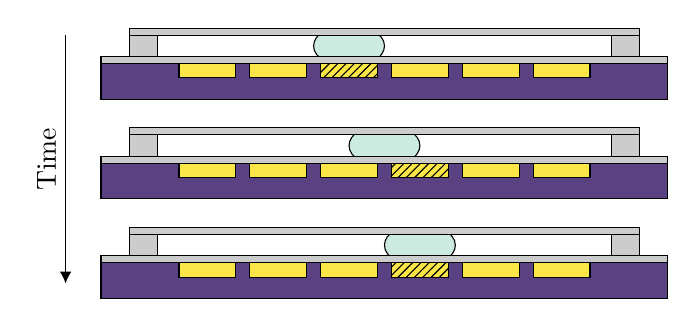
\begin{tikzpicture}[scale=0.09]
    \foreach \i/\activex in {0/30,1/40,2/40} {
      \begin{scope}[yshift=-400*\i]
        % draw the pcb
        \draw[fill=pd_purple] (0,0) rectangle +(80,5);
        % draw some electrodes
        \foreach \i in {10, 20, ..., 60} {
          \draw[fill=pd_gold] (\i+1,5) rectangle +(8,-2);
        }
        \draw[pattern=north east lines] (\activex+1,5) rectangle +(8,-2);

        % dielectric and hydrophobic layers
        \draw[fill=black!20] (0,5) rectangle +(80,1);

        % spacers
        \draw[fill=black!20] (4,6) rectangle +(4,3);
        \draw[fill=black!20] (76,6) rectangle +(-4,3);

        % top plate
        \draw[fill=black!20] (4,9) rectangle +(72,1);

        % use background layer so we don't clobber the stroke of the plates
        \begin{scope}[on background layer]
          \begin{scope} % make sure to clip in a new scope
            \clip (10,6) rectangle +(60, 3);
            \draw[fill=blue!40!green!20] (35,6) + (\i * 5, 1.5) circle [y radius=3, x radius=5];
          \end{scope}
        \end{scope}
      \end{scope}
    }
    \draw[->] (-5,9) -- node[rotate=90, above] {Time} +(0,-35);
  \end{tikzpicture}

  \caption{
    Side view of the PurpleDrop DMF device.
    Electrodes (yellow) sit at the top of the PCB (purple) in a grid.
    The PCB is topped with a dielectric and hydrophobic layer.
    The top plate sits on risers and is also hydrophobic and conductive.
    Droplets are attracted to the activated electrodes (shown with diagonal lines).
    Activating the neighboring electrode will move a droplet.
  }
  \label{fig:board-side}
\end{figure}

\subsection{Controlling DMF devices}
\label{sec:dmf-software}

The ``machine language'' that controls DMF devices is little more than turning individual electrodes on or off.
To move a droplet from one location to another, a controller must activate the electrodes along that path in sequence.
This sequence of electrode actuations explicitly refers to locations on the board, and there is no notion of the identity, properties, or even the existence of the droplets.
A better programming model allows high-level operations such as those shown in \autoref{fig:dag}, and the tool plans where those operations should occur and how the droplet operands get there.

Existing work has tackled these problems with place-and-route techniques from VLSI
\cite{bohringer2006parallel, grissom2012scheduling, yao2016contamination, zhao2012contamination, huang2010contamination, keszocze2015routing, roy2010routing, grissom2014interpreting}.
The input to these tools is a directed acyclic graph that encodes the data dependencies of the operations.
\autoref{fig:dag} shows a pseudo-code snippet along with the corresponding DAG.
Tools can take such a DAG and, together with the layout of the DMF chip, automatically determine when and where to execute each operation.
The tool then plans routes for every droplet so that they do not collide on the way.
Importantly, this is all done \emph{ahead of time}:
the tool statically determines if executing a given DAG on a given chip is possible.
However, DAGs do not naturally express constructs found in programming like conditionals, loops, or functions.

Other approaches have proposed domain specific languages (DSLs) to increase expressiveness~\cite{grissom2015open, grissom2014interpreting, curtis2018compiler, ott2018bioscript, biocoder}.
A DSL can support features like data-dependent control flow, which is necessary if a fluidic program is expected to act on the value of a sensor reading.
However, compiling or interpreting microfluidic programs in these languages introduces a fundamental trade-off between the flexibility of available programming constructs and the ability to statically reason about the program.
In order to statically place and route a protocol, a system must be able to prove the protocol only uses resources that the hardware can supply.
To meet this requirement, existing work has limited or eliminated programming features that allow potentially unbounded resource usage (e.g., loops, data structures, recursive functions, and error detection and recovery).

% dag figure
\begin{figure}
  \hfill
  \begin{minipage}{0.45\linewidth}
    \begin{lstlisting}[emphstyle=\underline, numbers=none, xleftmargin=0mm]
a = input(substance_A)
b = input(substance_B)
ab = mix(a, b)

heat(ab)
    \end{lstlisting}
  \end{minipage}
  \hfill
  \begin{minipage}{0.45\linewidth}
    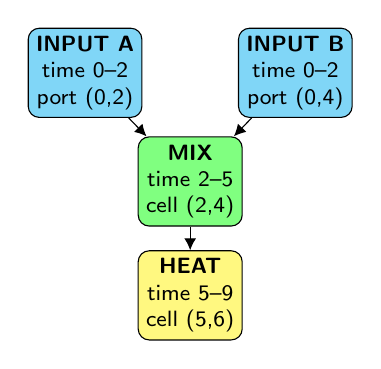
\begin{tikzpicture}[
        every node/.style={draw, align=center, rounded corners},
      ]
      \footnotesize \sf
      \node[draw=none] (mid) {};
      \node (A) [left = 5mm of mid, fill=cyan!50] {
        \textbf{INPUT A} \\
        time 0--2 \\
        port (0,2)
      };
      \node (B) [right = 5mm of mid, fill=cyan!50] {
        \textbf{INPUT B} \\
        time 0--2 \\
        port (0,4)
      };
      \node (mix) [below = 7mm of mid, fill=green!50] {
        \textbf{MIX} \\
        time 2--5 \\
        cell (2,4)
      };
      \node (heat) [below = 3mm of mix, fill=yellow!50] {
        \textbf{HEAT} \\
        time 5--9 \\
        cell (5,6)
      };

      \draw[->] (A) -- (mix);
      \draw[->] (B) -- (mix);
      \draw[->] (mix) -- (heat);
    \end{tikzpicture}
  \end{minipage}

  \caption{
    Pseudocode for fluidic a program fragment and the corresponding DAG where the operations have been
    scheduled and placed.
  }
\label{fig:dag}
\end{figure}

\section{Dynamic Microfluidic Programming}
\label{sec:programming}

\mw{say something about working with large droplets}

The vision put forward in this paper calls for a microfluidics platform that can combine computation and fluidic manipulation in an unrestricted, high-level programming model.
Our microfluidic programming system, Puddle, realizes this vision by making a different trade-off than previous work in microfluidics and doing everything dynamically.
This decision is based on the following key insight: when it comes to resource management, expressiveness comes from dynamism.
As a result, Puddle is not a programming language but a runtime system that provides a high-level API for microfluidic manipulations.
The runtime system dynamically manages the fluidic resources (droplets), imposing no restrictions on the user's programming model.

This section serves as an introduction to the Puddle API, detailing what it provides to the programmer and the runtime system implementer.
\autoref{sec:impl} explains the implementation,
and \autoref{sec:discussion} discusses the benefits and trade-offs of our approach.

\subsection{Example}

While the Puddle API is language-agnostic (we provide frontends in both Rust and Python), we focus on the Python frontend for this paper.
Python immediately satisfies many of the requirements for an effective microfluidic programming solution.
Python is popular with beginning programmers ~\cite{python-intro}, and it is also the language of choice for many scientists due to the wealth of libraries for scientific computation~\cite{scipy} and bioinformatics~\cite{biopython}.
Python also has a read-eval-print-loop (REPL), allowing users to interactively write (microfluidic or conventional) programs.

Consider the program snippet in \autoref{fig:code-mix-heat}.
Users write regular Python programs that interface with Puddle through a simple library that implements the Puddle API (fully described in \autoref{sec:api}).
Python snippets shown throughout the paper will have calls into Puddle underlined.

% code example
\begin{figure}
  \centering
  % \mw{check volumes here, make heat mutate}
\begin{lstlisting}[emphstyle=\underline, deletekeywords={temperature}]
# reduce is a functional fold over lists
from functools import reduce

def mix_n_heat(droplets):
    vol_before = sum(|\label{line:volume1}|
        d.volume for d in droplets
    )
    stuff = reduce(mix, droplets)
    stuff.heat(temp=90, seconds=60)
    if stuff.volume < vol_before: |\label{line:volume2}|
        print("we lost some volume!")
    return stuff

a = input("substance a", volume=1.0) |\label{line:start}|
b = input("substance b", volume=2.0)
c = input("substance c", volume=1.5)
abc = mix_n_heat([a, b, c])
\end{lstlisting}

  \caption{
    A example Python program interfacing with Puddle.
    Puddle API calls are underlined.
  }
  \label{fig:code-mix-heat}
\end{figure}


Starting at line \ref{line:start}, the user inputs three samples of various volumes.
These inputs take the substance name and requested volume of the sample.
Larger droplets may span multiple electrodes, but Puddle handles that automatically.
The \codeinline{input}s return opaque handles to the new droplets called \emph{droplet id}s.
The user then calls \codeinline{mix_n_heat} with a list containing the three droplet ids as an argument.
Note that \codeinline{mix_n_heat} is regular Python function and thus is completely transparent to the Puddle system; it could be recursive, exported or imported from a library, or passed around as a first-class value.

Inside \codeinline{mix_n_heat}, the user calculates the expected volume of mixing all the droplets together by adding their individual volumes.
The droplets are then all mixed together by reducing the list with \codeinline{mix}, resulting in a new droplet id \codeinline{stuff}.
The call to \codeinline{heat} then mutates \codeinline{stuff}.
The user then compares the droplet's new volume (which may have shrank due to evaporation) to the expected one, conditionally prints something, and then returns a handle to the mixed, heated droplet.

The API calls to \codeinline{input}, \codeinline{mix}, and \codeinline{heat} were \emph{non-blocking}.
They immediately returned new droplet ids without actually manifesting the droplets that those ids represent, which might take several seconds.
All manipulations and actuations are non-blocking in Puddle, because the user has no way to inspect their progress except through other API calls.
Non-blocking calls give the runtime system more flexibility in how to implement operations on the microfluidic device.
For example, even though \codeinline{mix} is binary in the API, the runtime system can see that the user intends to mix many droplets together, which could lead to more efficient execution.

In contrast, the accesses to \codeinline{volume} on lines \ref{line:volume1} and \ref{line:volume2} are blocking; they are also the only points at which something happens on the microfluidic device.
The volume of a droplet is a dynamic property: it cannot (in general) be known statically, as precision errors in \codeinline{input} and actuations like \codeinline{heat} might change it.
These calls must block and wait for the system to produce the relevant droplets and take the sensor reading, because the return value is just a number that the user's program (which Puddle knows nothing about) can manipulate and branch on.

\subsection{Programming Interface}
\label{sec:api}

\mw[inline]{make this longer, further describe the semantics}

The API's most important feature is that it deals in opaque handles to droplets called \emph{droplet ids}.
The user cannot introspect on these ids (they are just numbers), so all queries and manipulations of droplets must go through the API.
Therefore, Puddle is free to reorder, optimize, or delay performing the requested operations, allowing many calls in the API to be non-blocking.
This opacity also allows Puddle to provide automatic error correction and process-like isolation for concurrency.

% api figure
\begin{figure}
  % {\bf Manual droplet I/O}
  % create(location, dimensions, volume) $\to d$ \\
  % destroy($d$) \\
  \begin{minipage}[t]{.55\linewidth}
    {\bf Fluidic I/O} \\
    \codeinline{input}(name, volume) $\to d$ \\
    \codeinline{output}(name, $d$) \\

    {\bf Sensing} \\
    \codeinline{volume}($d$) $\to$ volume of $d$ \\
    \codeinline{temperature}($d$) $\to$ temp.\ of $d$
  \end{minipage}
  \begin{minipage}[t]{.42\linewidth}
    {\bf Fluidic Manipulation} \\
    \codeinline{mix}($d_1$, $d_2$) $\to d$ \\
    % \codeinline{combine_into}($d_1$, $d_2$) $\to d$ \\
    \codeinline{split}($d$) $\to$ ($d_1$, $d_2$) \\
    % \codeinline{move}($d$, location) $\to d'$ \\
    \codeinline{heat}($d$, temp, time) $\to d'$ \\

    {\bf Other} \\
    \codeinline{flush}($d_1, d_2, ...$)
  \end{minipage}
  \caption{
    The Puddle API.
    $d$s are droplet ids, opaque handles to droplets.
    All calls are non-blocking except for those under Sensing.
  }
  \label{fig:api}
\end{figure}

The complete Puddle API is listed in \autoref{fig:api}.
The calls for fluidic I/O and manipulation are non-blocking; they immediately return a fresh droplet id.
The fluidic I/O calls are indexed by a name, which refers to an input pump based on a configuration file with the hardware details.
The fluidic manipulation functions are self-explanatory.
Note that they are functional, consuming their droplet id arguments and returning new ones.
The frontend, however, is free to wrap the API calls to provide an idiomatic interface:
for example, \codeinline{heat} was used imperatively in \autoref{fig:code-mix-heat}.

% except for \codeinline{combine_into}, which is similar to \codeinline{mix} but guarantees that $d_1$ will not be moved until combined with $d_2$.
% This is useful for ``rescuing'' droplets that have become too small to move\footnotemark; see \autoref{sec:thermocycle} for an extended example.
% \footnotetext{On DMF devices, a droplet that is too small will be too far from its neighboring electrodes for the electrowetting force to move it.}

The sensing API calls force the system to ``flush the queue'' by performing the operations necessary to make the input droplet.
The \codeinline{volume} operation reads the volume using the camera (see \autoref{sec:vision}).
The \codeinline{temperature} operation measures the temperature using an onboard sensor.
In our Python frontend, \codeinline{volume} and \codeinline{temperature} are getters.

\camera{Add explanation of flushing multiple droplets.}
The \codeinline{flush} operation allows the user to manually force to realize the specified droplets (or all of them, if none are given), which is useful in interactive programming.
This can also be useful to inform Puddle of parallelism it would otherwise not see, as seen at the end of \autoref{sec:drawbacks}.

Users can easily extend the Puddle API with their own actuation and sensing primitives.
The mechanism for allocating space on the device (\autoref{sec:planning-planning}) is sufficiently general to implement any primitive that the hardware might support.

\subsection{Handling Errors}

API calls can fail instantaneously for two reasons: invalid arguments or using a consumed droplet id.
These failures happen as soon as the API call is made and are recoverable; the error propagates back to the user (in the form of an exception in the Python frontend).
Consider the following code snippets:

\begin{minipage}{.49\linewidth}
\begin{lstlisting}[numbers=none]
input("water", 1e-10)
\end{lstlisting}
\end{minipage}
\begin{minipage}{.49\linewidth}
\begin{lstlisting}[numbers=none]
ab = mix(a, b)
mix(ab, a)
\end{lstlisting}
\end{minipage}

The left snippet demonstrates an invalid argument by trying to \codeinline{input} too small a volume of fluid; the pumps do not have that level of precision.
The right snippet reuses droplet id \codeinline{a} after it has been consumed on the first line.
Droplets are physical resources that can only be consumed once.
All API calls under ``I/O'' and ``manipulation'' consume their droplet arguments.
It is the programmer's responsibility to not reuse droplets ids that have been consumed.
An imperative interface (like \codeinline{heat} in \autoref{fig:code-mix-heat}) can help prevent this problem by changing the droplet id that the wrapper object refers to.
The Rust frontend statically prevents droplet reuse through its ownership-based type system.

Additionally, hardware failures may occur during execution, making droplets not move or actuate as planned.
\camera{Clarified the situation in which errors are unrecoverable}
Most of these are automatically detected and corrected by Puddle's error correction system (described in \autoref{sec:vision}).
In rare cases, however, an error can result in a situation that is unrecoverable (e.g. the number of failed electrodes prevents routing).
Because actuation API calls are non-blocking, the program may have progressed with the assumption that the promised droplets will be actually produced.
Therefore, Puddle treats this case as unrecoverable and throws an exception to the user.

% A more subtle case occurs when a droplet leaves the safe volume range, perhaps due to evaporation from heating.
% Droplets that are too small cannot move on DMF devices, so Puddle sends an exception back to the user.
% This exception differs from those in the previous paragraph because it originates from a non-blocking call, so the user may have to handle it anywhere.
% The \codeinline{flush} operation gives the user control over when execution occurs on the DMF device, so it provides a single point from which these exceptions can be handled.
% \autoref{sec:thermocycle} demonstrates an example of this kind of error handling.

% Internally, these ids are associated with various physical properties of the droplets needed for routing: the location of the droplet, its dimensions, and its volume.
% All droplets are assumed to be rectangular for, or at least we only use rectangular actuation patterns.
% The location and the dimensions of the droplets are given as integer (y,x) coordinates.

\camera[inline]{
  The subsection ``Implications of Dynamism'' has been moved and broken down
  into the new discussion section to clarify the fact that the points made there
  are intended for insight and discussion rather than contribution claims.
}

\section{Implementation}
\label{sec:impl}

Our implementation spans three levels of the stack shown in \autoref{fig:stack}: a frontend that facilitates high-level microfluidic programming against the Puddle API, the Puddle runtime system which implements the API detailed in \autoref{sec:api}, and PurpleDrop, the DMF device which Puddle controls.
The interface and programming model were covered in the previous section; here we detail the implementation of the hardware and runtime system.

% The Puddle API deals principally with opaque handles to droplets called \emph{droplet id}s.
% Much like file descriptors discussed above, the opacity of droplet ids abstracts away low-level details like the droplet's location, and forces all interaction through the API.
% Users can program with Puddle using any language they like; they just need a simple library can than communicate with Puddle over JSON.
% These programs can therefore run directly on the Raspberry Pi or on a remote machine with greater computational power.


\subsection{PurpleDrop DMF Device}

\begin{figure}
  \centering
  \begin{tikzpicture} [
        box/.style={draw, fill=white, align=center, rounded corners},
    ]
    \sffamily
    \node[anchor=south west,inner sep=0] at (0,0) {
      \includegraphics[width=\linewidth]{purpledrop.jpg}
    };
    \node[box] (base) at (1.6, 1.5) {A};
    \node[box] (cart) at (3.0, 1.8) {B};
    \node[box, anchor=center] (heaters) at (4.38,1.5) {C};
    \node[box] (pump) at (1, 2.7) {D};
    \node[box] (input) at (3.5, 2.9) {E};
    \node[box] (pi-pins) at (4.1, 5.5) {F};
    \node[box] (cam) at (5.6, 4.5) {G};

    \node (h1) at (3.80, 2.31) {};
    \node (h2) at (4.38, 2.31) {};
    \node (h3) at (4.96, 2.31) {};

    \path[->]
      ([xshift=-2]heaters.north) edge[out=90, in=270] (h1)
      (heaters) edge[out=90, in=270] (h2)
      ([xshift=2]heaters.north) edge[out=90, in=270] (h3)
      ;

  \end{tikzpicture}
  \caption{
    PurpleDrop, our digital microfluidic device.
    The motherboard PCB ({\sf A}) contains the electronic components, and the daughterboard ({\sf B}) contains the electrodes and the hydrophobic surface detailed in \autoref{fig:board-side}.
    The device supports heaters on the bottom three electrodes ({\sf C}).
    We can drive up to three pumps ({\sf D}) that can input or output fluids on the edge of the device ({\sf E}).
    PurpleDrop is controlled by a Raspberry Pi over the 40-pin connector ({\sf F}).
    The Raspberry Pi connects to a camera on a 3D-printed mount (\sf G).
  }
  \label{fig:purpledrop}

\end{figure}

We designed our digital microfluidic device, PurpleDrop, with simplicity and accessibility in mind.
All together, the components cost on the order of \$300, orders of magnitude less than most other microfluidic systems.
Furthermore, the design uses commodity components and does not require a clean room, so anyone with electronics experience could assemble PurpleDrop on their own or have it assembled by a PCB assembly service.
\autoref{fig:purpledrop} shows the device and enumerates its components.

\paragraph{DMF hardware}

The DMF portion of PurpleDrop is responsible for holding and manipulating the droplets.
The daughterboard contains the electrodes that hold the droplets, and the motherboard contains the electrical components such as high-voltage controllers, shift registers, etc.
Both mother and daughterboard are PCBs.
The daughterboard is removable, allowing different configurations of electrodes with the same motherboard.
The modularity is also useful for durability, as the daughterboard is the most prone to wear.

PurpleDrop's design was inspired by OpenDrop \cite{opendrop}, an existing open-source DMF platform.
Unlike OpenDrop, PurpleDrop runs without an oil medium for easier setup.
\autoref{fig:board-side} shows a side view of the PurpleDrop daughterboard.

\paragraph{Electronic control}

Instead of using a microcontroller to drive the electronics needed for electrowetting, we use a Raspberry Pi 3B \cite{raspberry-pi-3b} single-board computer.
The Raspberry Pi runs Linux and sports a quad-core 1.2 GHz ARMv7 processor as well as GPIO pins, allowing PurpleDrop to be a self-sufficient microfluidics platform.
The control software actuates the electrodes on the daughterboard with the GPIO pins through some shift registers on the motherboard.
The execution planning (\autoref{sec:planning}) and computer vision for error correction (\autoref{sec:vision}) also run on-device, so no host machine is needed.

\paragraph{Peripherals}

Microfluidic devices can move and mix liquid samples, but possible applications are limited without the ability to sense and manipulate properties of the droplets and get droplets to and from the device.
PurpleDrop includes a heater, temperature sensor, and the ability to do both input and output of droplets.
Input and output are driven by small peristaltic pumps which carry droplets to/from test tube reservoirs or other devices.
\autoref{sec:nanopore} demonstrates using fluidic IO to interface with a DNA sequencer.

PurpleDrop also uses a camera mounted on top of the device as a multi-purpose sensor.
The camera detects the locations of the droplets for error correction.
Other approaches like capacitive sensing \cite{bhattacharjee2012capacitance} would increase the hardware cost, where as the camera is relatively cheap.
The camera can also sense the volume of droplets, which is useful for certain protocols like that shown in \autoref{sec:thermocycle}.
Droplet volume is computed by multiplying the area of the droplet in the image by the fixed distance between the board and the top plate (see \autoref{fig:board-side}).

\subsection{Planning and Execution}
\label{sec:planning}

% planning flow
\begin{figure}
  \resizebox{\linewidth}{!}{%
    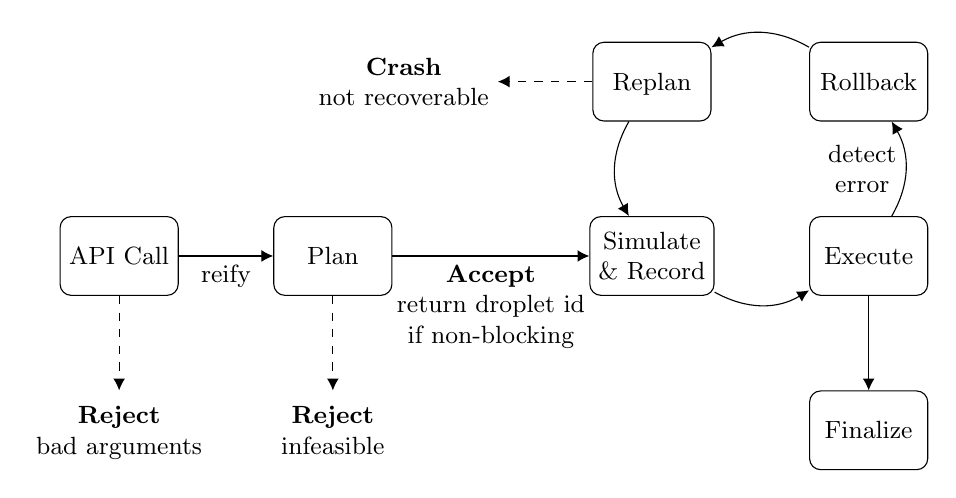
\begin{tikzpicture}[
      node distance = 12mm,
      every node/.style={
        align=center,
        text depth=0cm, % dont change box size base on letters
      },
      box/.style={draw,
        rounded corners,
        minimum width=1.5cm,
        minimum height=1cm,
      },
      outcome/.style={
        minimum height=1cm,
      },
      ]
      \small
      \node[box] (api) {API Call};
      \node[box, right=of api] (plan) {Plan};
      \node[box, right=2.5cm of plan] (sim) {Simulate \\ \& Record};
      \node[box, right=of sim] (exec) {Execute};
      \node[box, above=of exec] (roll) {Rollback};
      \node[box, above=of sim] (replan) {Replan};
      \node[box, below=of exec] (final) {Finalize};

      \node[outcome, below=of api] (api-reject) {{\bf Reject} \\ bad arguments};
      \node[outcome, below=of plan] (plan-reject) {{\bf Reject} \\ infeasible};
      \node[outcome, left=of replan] (replan-reject) {{\bf Crash} \\ not recoverable};

      \path[->]
      (api) edge node[below] {reify} (plan)
      (plan) edge node[below] {{\bf Accept} \\ return droplet id \\ if non-blocking} (sim)
      (exec) edge (final)

      (sim) edge[bend right] (exec)
      (exec) edge[bend right] node[left] {detect \\ error} (roll)
      (roll) edge[bend right] (replan)
      (replan) edge[bend right] (sim)

      (api) edge[dashed] (api-reject)
      (plan) edge[dashed] (plan-reject)
      (replan) edge[dashed] (replan-reject)
      ;
    \end{tikzpicture}
  }
  \caption{
    The life of a command.
    Dashed edges end the flow immediately.
    Commands may be rejected if the API call was malformed or a feasible execution plan cannot be found.
    The user can recover from rejected commands, but not from failures to replan accepted ones.
  }
  \label{fig:planning}
\end{figure}

Because all the complications of a programming language (loops, function calls, conditionals) are handled at the user level, the internals of Puddle are concerned only with the planning and execution of API calls.
Note that we do not use any of the existing algorithms that might guarantee optimal routing or extract parallelism.
This decision was made primarily to simplify implementation, but also because none of our microfluidic needs demand that level of efficiency.
\autoref{sec:future} discusses how we could incorporate this body of work into our system.

\autoref{fig:planning} shows the entire lifetime of an API call.
The first step is reification into a \emph{command}, the object used internally to represent a request from the user.
The remainder of the flow operates on these command objects.
All types of commands (input/output, sensing, actuation) go through the same flow, so a user can extend Puddle with a new primitive without modifying the planning and execution infrastructure.

\subsubsection{API Calls to Commands}

Commands store the operations' arguments, input droplet ids, and freshly created output droplet ids for droplet manipulation operations.
These output droplet ids correspond to the droplets that command will make if successfully executed.
After the command is created and planned, the system can return these ids if the API call was non-blocking, allowing the program to proceed without waiting on execution.

% cmd creation can fail

The core of planning is placement and routing, which occur after the API call has been reified into a command.
Commands can form a DAG where the edges are their droplet id dependencies.
For simplicity, however, we store them in a queue and place and route them serially.

\subsubsection{Planning}
\label{sec:planning-planning}

Each command makes an \emph{allocation request} for space on the microfluidic board.
For example, \codeinline{mix} requests a rectangle slightly larger than the resulting combined droplet so it has space to move the droplet in a circle, agitating the mixture.
The allocation request can also place constraints on the features of the space, e.g. \codeinline{heat} requests a space with a heater.
Our simple placement algorithm directly checks for the best of all possible ways to satisfy a location.
This is linear in the size of the hardware, and the hardware is small, so practically we can still do this in real-time.

The allocation request also specifies the (relative) desired locations of the input droplets.
In the case of mixing two $1 \times 1$ droplets, \codeinline{mix} will request a $3 \times 2$ rectangle and ask that the input droplets start at coordinates $(0,0)$ and $(1,0)$.
The adjacent droplets will combine, leaving a $2 \times 1$ droplet inside the $3 \times 2$ rectangle.
After the allocation request is placed, the system routes the input droplets to their specified locations using a modified A* algorithm \cite{a-star, bohringer2006parallel}.
Both placement and routing ensure that droplets stay at least 1 space apart to avoid collisions.

If either placement or routing fails, the command is rejected as infeasible.
Because planning happens right after command creation, the user gets an immediate, recoverable error.
If planning succeeds, then non-blocking API calls can return droplet id(s) knowing that their successful execution is at least feasible (although not guaranteed in the face of hardware errors).

\subsubsection{Simulation and Recording}
\label{sec:simulation}

Regardless of whether the API call is blocking, successfully planned commands are then simulated.
Each time step in the simulation is recorded, resulting in a \emph{record} of where each droplet is (and thus which electrodes to activate) at every moment.
The record provides a view into the future state of the microfluidic device assuming that no hardware errors occur during execution.

\camera[inline]{Clarified some aspects of simulation.}
Puddle only simulates droplet movement to check for errors and determine the presence and location of droplets on the DMF device at each timestep.
Chemical results of actuations on the droplets or mixing them are not simulated.
Simulation does, however, record when actuations occur, so execution can perform them when it ``replays'' the record.

The record allows multiple commands to be planned ahead-of-time without executing any of them.
Consider the following program snippet:

\begin{lstlisting}[emphstyle=\underline, numbers=none, xleftmargin=15mm]
for i in range(1000000):
    input("water", volume=3.0)
\end{lstlisting}

This program clearly cannot run on our microfluidic hardware; it requires more space than any DMF device available today.
And since Puddle knows nothing about the program structure, it will begin to accept these operations as they are submitted.
However, commands are planned with respect to the latest state in the record, i.e. commands are planned under the assumption that all previous commands execute exactly as planned.
Eventually, one of the \codeinline{input}s in the above program will be infeasible, since the DMF device will be full of the previous droplets.
Puddle will reject the command as infeasible, returning an error to the user even though none of the commands have been executed yet.

\subsubsection{Execution, Monitoring, and Rollback}

The simulation record allows execution to be asynchronous with planning.
Execution simply consists of popping the earliest state from the record, and activating the electrodes (and any peripherals) according to the droplets' position in that state.
After a short delay, Puddle uses its computer vision system (described in \autoref{sec:vision}) to detect the actual state of droplets on the device.
If the actual state does not match the expected state, the system triggers a rollback.
\camera{Cited some relevant work on error correction.}
This ``check and correct'' flow is similar to previous work \cite{hu2013fault} that uses capacitance sensing instead of computer vision.

A rollback consists of deleting the record and replanning all commands which have not been completed.
Replanning is identical to planning, except that failure to \emph{re}plan is unrecoverable (\autoref{fig:planning}).
Non-blocking API calls may have already returned with a droplet id that essentially promises that new droplet.
Since Puddle had no knowledge of the program, we have no choice but to terminate.

During the rollback, Puddle can also mark any electrodes that failed to move a droplet as dead.
% \karin{or schedule to perform testing routines on those electrodes later to determine if the failure was permanent}
Otherwise, the rollback would replan the same route over the same electrode, and the error would occur again.
\autoref{sec:endurance} demonstrates how this allows execution on a DMF with faulty electrodes.
The user can tune this behavior, forcing Puddle to retry an electrode a certain number of times before marking it as dead.

Replanning can fail in one of two cases: the number/identity of the droplets on the board has suddenly changed (something accidentally mixed), or the new arrangement of droplets is impossible to place and route.
The first case is relatively unlikely, as hardware errors tend to be a failure to move a droplet (due to some defect with the DMF device) rather than an errant move in some other direction.
The second case is also unlikely in the face of few errors: the main constraints to placement and routing are the number of droplets on the device, and the same droplets (albeit in a different arrangement) were successfully planned before.
However, as errors accumulate, Puddle avoids more and more regions of the board.
If enough errors build up, routing can become impossible, and replanning will fail.

The record also keeps track of the states that commands were completed in.
When execution reaches such a state, the command is finalized.
For most commands, this does nothing, but for blocking commands, this sends the result back to the user.

\subsection{Error Detection via Computer Vision}
\label{sec:vision}

\begin{figure}
  \centering
  \includegraphics[width=0.6\linewidth]{droplet-vision}
  \caption{
    A computer vision system identifies droplets in real time for error detection and volume measurement.
  }
  \label{fig:tracking}
\end{figure}

The previous section discussed how Puddle corrects errors via the rollback and replan mechanism, but not how we detect them.
Like other works, we use a computer vision system to localize the droplets on the DMF device.
However, our system is more flexible.
Past work has required either a template image for a droplet~\cite{luo2013error} or a reference background image of the electrode array~\cite{shin2010vision, vo2017image-dmf}.
The template image approach does not scale to droplets of different shapes and sizes, and the background difference approach is sensitive to changes in lighting and therefore requires a highly controlled environment.

We detect droplets based on color.
We tint all the input fluids with green dye, and then calibrate the vision system to that hue.
Any object within that hue range is recognized as a droplet.
Because we are using the hue-saturation-value color space, our system is resistant to changes in lighting.
We require only a simple paper shade to reduce glare off of the reflective surface of the chip.

The shape detection portion of error detection is implemented in OpenCV \cite{opencv}.
The result of the hue filtering is a binary image indicating which pixels are the desired shade of green.
A series of morphological operations (erosions and dilations) suffices to remove any noise.
A contour finding algorithm \cite{findcontours} then generates shapes that represent the droplets.
We finally use a projective transform to map those shapes from the image's coordinate space to that of the DMF device.

Once the shapes are detected, Puddle must determine if the set of shapes constitutes an error.
The first step is to match the shapes with the expected droplets.
We use a distance metric to measure the difference in their locations and sizes.
The pairwise distances form a bipartite graph, and we find a matching using the Kuhn-Munkres algorithm \cite{munkres}.
Each shape is then compared with its expected droplet.
If they are all similar enough, execution proceeds.
If there is a significant difference between the expectation and reality according to the camera, we convert the shapes into the new expected state and trigger a rollback, which replans unfinished commands starting from the new state.

The result is an error detection system that is more robust to lighting changes and handles droplets of any shape or size, an improvement over previous work.


\section{Evaluation}
\label{sec:eval}

We evaluate our system both quantitatively and qualitatively.
First we evaluate the computer vision system in isolation, then we evaluate it in the context of error detection and correction.
We then demonstrate Puddle's ability to write high-level programs and interface with other computer systems with two case studies.

\subsection{Computer Vision}
\label{sec:vision-eval}

\begin{table}
  \centering
  \begin{tabular}{lr}
    \bf Image Segmentation Metrics \\
    Mean Precision & 0.9851 \\
    Mean Recall & 0.9147 \\
    Mean False Positive Rate & 0.0001 \\
    \\
    \bf Droplet Metrics \\
    Mean accuracy of droplet area & 0.9220  \\
    Incorrect droplet count & 1 / 57 \\
    Droplet occupation overestimates & 14 / 56 \\
    Droplet occupation underestimates & 0 / 56 \\
  \end{tabular}
  \caption{
    Results from evaluating our computer vision system on 57 manually labeled images of the DMF device.
    The first set of metrics come from image segmentation, and the second set is specific to droplet recognition.
    Droplet occupation is explained in \autoref{sec:vision-eval}.
  }
  \label{tab:vision-results}
\end{table}

We evaluated our computer vision system on a dataset of 57 images taken from the Raspberry Pi camera at 320x240 pixels, the resolution we use for real time tracking.
We manually labeled the droplets in the image and also specified which electrodes they occupied.
The images cover a wide variety of droplet counts, droplet locations, and droplet areas on the microfluidic board, and are thus representative of the microfluidic setup, and the variability expected to arise within the setup during normal operation of the device.
We used a single piece of white paper mounted above the device to reduce the glare off the PCB, otherwise the lighting was uncontrolled and varies throughout the images.

\autoref{tab:vision-results} shows the results of our evaluation.
Since droplet recognition is similar to image segmentation, we first calculate some metrics from that domain.
Notably, the precision is higher than recall, indicating that our recognition system is relatively conservative.
This comes from the fact that our system uses more erosion than dilation to remove noise from the image.
Erosion results in slightly smaller recognized areas in the image, whereas too much dilation would combine nearby droplets.
The area underestimate is consistent and thus could be calibrated out.

We also compute a number of metrics specific to droplet recognition.
Droplet count is the most important metric for error correction.
If the system observes the wrong number of droplets, it cannot match the expected state to the actual state.
We only saw one of these errors in the dataset: in an image with droplets on neighboring electrodes, the system confused two droplets as one.
Puddle prevents droplets from being on neighboring electrodes to avoid accidental mixing, so this error is unlikely to occur in practice.
Of the remaining 56 images, we calculated the electrodes the droplets occupied.
Puddle takes a conservative approach here, preferring to turn on more electrodes rather than fewer to ensure droplet movement.
The results reflect this with 14 overestimates but no underestimates.
Overall, these results indicate that the vision system allows for correct and reliable droplet detection.

\subsection{Error Correction}
\label{sec:endurance}

% endurance figure
\begin{figure}
  \centering
  \begin{tikzpicture}
    \datavisualization [
      scientific axes,
      x axis={
        length=0.8\linewidth,
        ticks={step=2},
        include value=0,
        label=Circle around board
      },
      y axis={
        length=3cm,
        ticks={step=2},
        label=Cumulative errors corrected
      },
      visualize as line
    ]
    data[headline={x, y}, read from file=data/endurance.csv];
  \end{tikzpicture}
  \caption{
    To test error correction, we moved a droplet in circles until failure.
    Total experiment time was 2 hours and 11 minutes.
    Along the way, the computer vision system detected and corrected errors, marking regions of the board as faulty and avoiding them in the future.
    The errors at the beginning correspond to faulty electrodes; those at the end were caused as the droplet evaporated.
  }
  \label{fig:endurance}
\end{figure}

In Puddle, we use the droplet position and size information as part of a larger error correction system including droplet matching, rollback, and replanning (detailed in \autoref{sec:planning}).
To evaluate these mechanisms and their impact on DMF reliability, we staged an endurance test on the microfluidic device.

DMFs can suffer from either inherent or use-induced failure.
Flaws inherent to the device itself, e.g., surface flaws or poor electrical contact in the wiring for some electrodes, lead to failure early in execution.
Use-induced defects, e.g., droplet evaporation or surface wear, lead to failure later in execution.
Our endurance test demonstrates that Puddle's error correction can extend the life of a DMF device, allowing it to run longer protocols in the face of both types of failure.
We specify four points on the chip near the corners and route a droplet between them over and over until the system eventually marks so many electrodes as faulty that routing fails.

\autoref{fig:endurance} shows the results of our endurance test.
Note that six errors occur relatively soon in the test, before the completion of the fourth loop.
Without error correction, a protocol would be forced to terminate here.
These errors were due to poor electrical contact, resulting in a weaker electrowetting force that failed to pull the droplet to that electrode.
Our error correction system identified these electrodes and avoided them in later loops.
The later errors (starting around loop 34) were due to evaporation, leaving the droplet too small to move reliably.
The next section demonstrates how automatic replenishment can deal with evaporation.

\subsection{PCR and Thermocycling}
\label{sec:thermocycle}

% thermocycle code
\begin{figure}
  \centering
\begin{lstlisting}[basicstyle=\ttfamily\small]
min_volume = 10 * microliters

def thermocycle(droplet, temps_and_times):
    for temp, time in temps_and_times:
        heat(droplet, temp, time)
        if droplet.volume < min_volume
            # '+=' is a mutating mix
            droplet += input("water", min_volume)

def pcr(droplet, n_iter):
    thermocycle(droplet, n_iter * [
        (95,  3 * minutes),
        (62, 30 * seconds),
        (72, 20 * seconds),
    ])
\end{lstlisting}
  \caption{
    Python code for polymerase chain reaction (PCR) and thermocycle.
    The heating in thermocycling can evaporate droplets, so the code replenishes with water if necessary.
    Note that list multiplication in Python is concatenation, e.g. \codeinline{2 * [1] == [1, 1]}
  }
  \label{fig:thermocycle-code}
\end{figure}

Many chemical or biological protocols include thermocycling, or repeated heating and cooling, to speed up a reaction or denature a reagent.
Thermocycling poses a challenge to current DMF systems that operate in air (as opposed to oil):
The heating portion of thermocycling could evaporate the small droplets being manipulated on the DMF device.

From a programming perspective, the natural way to express thermocycling is with a loop.
Moreover, thermocycling is not a protocol in itself, but rather it is an important part of many other protocols.
Ideally, we would write the code for thermocycling once, and its behavior would be parameterizable and reusable.

\autoref{fig:thermocycle-code} shows our implementation of thermocycling in Puddle.
The use of functions, data structures, and data-dependent control-flow put this implementation out of reach for any other high-level microfluidic programming system that we know of.

We also implemented polymerase chain reaction (PCR) using \codeinline{thermocycle} as subroutine.
PCR is an important protocol in synthetic biology that selectively amplifies DNA in a solution.
We validated the experiment by using the Qubit system~\cite{qubit} to quantify the amount of DNA before and after amplification.
We performed 8 cycles of PCR which required 2 replenishments to avoid evaporation.
The procedure doubled the amount of DNA in our 10 microliter sample.
While commercial PCR instruments achieve more efficient amplification, our PCR protocol was successful and can be improved with more precise heaters and temperature sensors.
%Our PCR was therefore successful but inefficient (industrial PCR equipment achieves higher amplification), likely due to imprecision in heating the droplets.
To our knowledge, this is the first fully-automated execution of PCR with replenishment on a DMF device in air.


\subsection{DNA Sequencing}
\label{sec:nanopore}

\begin{figure}
\begin{lstlisting}[basicstyle=\ttfamily\small]
def sequence(droplet):
    # actual prep protocol
    droplet += input("buffer", 65 * microliters)
    output("sequencer", droplet)
    # pseudocode to get and process the data
    data = get_data_from_device()
    seq = process(data)
    return seq
\end{lstlisting}
  \caption{
    A Python function that takes in a droplet and returns the sequence of DNA contained in that droplet.
  }
  \label{fig:nanopore-code}
\end{figure}

To further highlight the combination of microfluidic manipulation and computation, we performed DNA sequencing using Puddle and the MinION sequencer \cite{minion}.
The MinION requires some fluidic steps to prepare a sample for sequencing, and the raw output data requires processing to return the DNA sequence.
Because of the computation needed for data processing, the sequencer is connected directly to a laptop instead of the Raspberry Pi.
The Python code (including data processing) runs on the laptop, but the Puddle system still runs on the Raspberry Pi.
The two sides communicate over the network using the same Puddle API, which is encoded in JSON format.

The code for the sequencing protocol is listed in \autoref{fig:nanopore-code}.
\codeinline{get_data_from_device} and \codeinline{process_data} are pseudocode Python functions that get and process the data from the MinION; the former returns the raw data and the latter returns the actual DNA sequence.
We use pseudocode because the actual process for sequencing and processing involves a closed-source GUI application.
Given an API to perform these operations, automating the entire protocol including data acquisition and analysis is a matter of implementation.
We validated the DNA sequencing results from the experiment by comparing the reported sequences with the known sequences used as input.

The protocol is simple, but it still demonstrates the power of the Puddle programming model.
In one sense, the function \codeinline{sequence} is no more exciting than one that reads the contents of a file from disk.
However, existing microfluidic programming models cannot express both the fluidic and computational aspects of this protocol, nor can they export this functionality as an easy-to-use (and reuse) Python function.
To our knowledge, this is the first time that computation and protocol execution are merged in this way.
We envision encouraging the use microfluidics for complex experiment automation.

\section{Related Work}
\label{sec:related-work}

\paragraph{DMF hardware}
DMF devices can be built on different substrates including silicon, or on a printed circuit board (PCB).
While the former two technologies offer great control over the surface topology (an important property for electrowetting), PCBs are much more flexible and accessible, as they are cheaper and offer multi-layer wire routing \cite{gong2008direct}.
We chose a PCB substrate and operate in air because it makes the device easier to manufacture and use.
Our error correction system compensates for faults which may occur due to the more affordable substrate.

Jebrail et al. have presented a system for replenishing liquid on a DMF device~\cite{jebrail2015solvent}, but the intervention is not automated (a user manually pushed a syringe).

\paragraph{DMF routing}

Extensive work in this area has led to algorithms that can
exploit parallelism \cite{bohringer2006parallel, grissom2012scheduling},
reduce contamination \cite{yao2016contamination, zhao2012contamination, huang2010contamination},
and minimize overall droplet travel \cite{keszocze2015routing, roy2010routing}.
Our place and route algorithms in Puddle are intentionally very simple and do not provide these features, as these are outside the scope of this work.
\autoref{sec:future} discusses how such features could be implemented within our system.

\paragraph{Microfluidic Programming}
Previous work has improved upon static DAG place and route with domain specific languages for protocol specification and execution.
Grissom et al. propose a dynamic interpretation approach that allows control flow~\cite{grissom2014interpreting}, but the programming model is still centered around explicit DAG construction.
Dynamic interpretation also suffers from sub-optimal place and route, as the system only considers one basic block at a time.
Others have proposed static compilers capable of handling control flow, e.g., Curtis et al.~\cite{curtis2018compiler} and Ott et al.~\cite{ott2018bioscript}.
These approaches offer a static guarantee that the program (ignoring errors) can be successfully routed, but they are all less expressive than Puddle.
In particular, programs cannot (in general) use recursion, manipulate data structures, or allocate in loops.
The example given in \autoref{fig:thermocycle-code} exhibits the latter two of these characteristics.

Previous approaches using general purpose languages either offer little abstraction, requiring the user to manually address droplet locations~\cite{opendrop, dropbot}, or require re-expression in a restricted embedded DSL or manual DAG construction~\cite{curtis2018compiler, biocoder}.

Amin et al. propose an instruction set for a channel-based microfluidic architecture~\cite{amin2007aquacore}.
Puddle could feasibly target channel-based devices through such an ISA.

Autoprotocol \cite{autoprotocol} and Aquarium \cite{aquarium} focus on off-premises execution where users send samples and protocols to be executed by pipetting robots (Autoprotocol) or by human technicians (Aquarium).
Antha \cite{antha} targets various lab automation technologies for on-premises execution but not DMF.
The intended use case for these platforms is high-throughput fluidics rather than writing and running expressive programs.
In principle, Puddle could be used as a backend for these frameworks to allow execution on DMF devices like PurpleDrop.

% \paragraph{}
% This seems to suggest that programs will be executed with no idea of whether they can actually be run on the hardware, or that execution will be horrendously inefficient.
% These criticisms hold merit, but we can at least mitigate both problems (\autoref{??}).
% More importantly, while they are the subject of much research, these problems have yet to arise in our experience.
% We do not intend for our system to compete with works that compare how many droplets can be routed in a small space, or how many timesteps their simulations take.

% Our system was designed with the realization that our needs for a microfluidic programming platform were very simple in terms of fluidic complexity, and existing solutions didn't address the mixture of microfluidic and conventional programming.
% This is not a dismissal of past efforts in this area; in fact most of them tackle the algorithmic challenges far more efficiently than we do, and our framework could certainly benefit from integrating some of those solutions in.

% On the other hand, static place-and-route techniques cannot offer error correction or data-dependent control flow.
% For example, if the hardware fails when the controller attempts to move a droplet, a static execution plan will just continue, and the plan's model of chip will fall out-of-sync with reality.
% If a program branches on the value of a sensor reading, static execution planning gets more complicated.
% Simple conditionals can be handled by ``compiling'' basic blocks, but loops and procedures are still out of reach, as there's no ``stack'' on which to dynamically allocation droplets that might be created.

\paragraph{Error Correction for DMFs}

\autoref{sec:vision} mentioned that previous work on optical error detection is not as flexible as our approach in terms of droplet size/shape \cite{luo2013error} or lighting conditions \cite{shin2010vision, vo2017image-dmf}.
We do require that droplets are dyed green.
We are working to lift this restriction, as it limits the use of the camera as a colormetric sensor in the visible light spectrum.
Other work has proposed impedence sensing as a means of detecting droplets~ \cite{hadwen2012impedence}.

Alistar et al.\ \cite{alistar2010variability} present an ahead-of-time solution for operations that take variable time, accounting for some classes of precision errors.
An online solution has also been presented \cite{alistar2012online}, but it has an offline component and only works for programs represented as DAGs.
Previous work has also proposed error correction for DMF devices \cite{xu2008defect, xu2008defectplacement, hu2013fault, hsieh2014biochip, jaress2015online}, but these were implemented outside of a larger microfluidic programming solution, relied on more expensive sensors, or were only simulated.

\paragraph{Lazy dataflow processing}
\camera{Note some similarities to other frameworks as mentioned in the rebuttal}

Our approach of allowing the programmer to lazily manipulate opaque ids through an API bears a similarity to an approach used in data processing.
In particular, Apache Spark \cite{spark} and PyTorch \cite{pytorch} provide a similar abstraction for the domains of data processing and machine learning.
Both allow the user to build up sets of operations in a general-purpose host language, and then (upon request for data) a runtime system optimizes and executes the dataflow graph of pending operations.


\section{Discussion}
\label{sec:discussion}

\camera[inline]{This section has been moved to discussion, further highlighting the drawbacks of the purely dynamic approach.}

Our main contribution is the notion of a microfluidic runtime system that dynamically manages fluidic resources.
This advances upon previous work by allowing unrestricted flexibility and expressiveness, at the cost of some static guarantees.
Below we further detail the benefits of and reasons for this approach, discuss the drawbacks, and propose future work based on this key idea.

\subsection{Benefits of Dynamism}
\label{sec:benefits}

Existing work has approached microfluidic programming from the perspective that fluidic resources should be statically managed.
This provides guarantees that a program will ``fit'' on the microfluidic device, but limits the expressive power of the programming model.
Specifically, any programming feature that allows for potentially unbounded fluidic resource usage must be either prohibited or restricted, as the tool cannot statically perform place and route.

General-purpose computation has taken the opposite tack.
Nearly all of the abstractions that make up the modern computing stack (virtual memory, stack, heap, processes, file systems, etc.) provide the illusion of exclusive access and unlimited resources.
The systems under these abstractions cannot statically promise that enough resources exist, but their popularity demonstrates the value of favoring expressiveness over static safety.
\camera{Removed the claim about ``best effort'' policy of resource allocation}
Barring the development and use of sufficiently complex static analyses, existing fluidic programming systems cannot coexist with general purpose computation: one side wants to make promises that the other has given up on.

Puddle's design draws more inspiration from general purpose computer systems than synthesis tools for microfluidics.
Instead of trying to provide a monolithic solution, Puddle instead defines a small API that decouples fluidic management from the act of programming.
This design leads to many benefits that, to our knowledge, no other DMF programming system has.

Most importantly, Puddle abstracts away fluid management without restricting the programming model.
This flexibility is important since our target domains (automated experimentation, molecular computer systems, etc.) are new and have not yet settled on abstractions.
The separation of concerns in our approach allows the frontend(s) and the runtime system to advance independently.

The notion of opaque handles (droplet ids) representing dynamically managed resources (droplets) lets Puddle provide many features familiar to computer systems with very little effort.
Like the abstractions mentioned above, Puddle lets the user pretend they have unlimited resources (space on the microfluidic board) and exclusive access to it.
Puddle can provide process-like isolation by simply name-spacing droplet ids with a UUID, so multiple programs can run on a single device concurrently.
The Puddle API can also be used locally (on the Raspberry Pi) or remotely, useful for interactive programming or protocols that require heavy data analysis, respectively.

Unlike static approaches to digital microfluidic programming \cite{grissom2014interpreting, ott2018bioscript, curtis2018compiler}, dynamism also allows for metaprogramming.
Users can use features of their favorite languages (reflection, macros, first-class functions, etc.) to programmatically construct protocols.

Error correction is also closely tied to our dynamic approach.
Puddle implements error detection and correction using a computer vision system (details in \autoref{sec:vision}).
Abstract droplet ids allow the runtime system to freely move droplets around to correct and avoid errors.
Since the nature of a hardware failure cannot be known ahead of time, even static approaches to microfluidic programming that include this kind of error correction must resort to dynamic replanning, limiting the static promises that can be made in the face of errors.


\subsection{Drawbacks of Dynamism}
\label{sec:drawbacks}

These benefits come with a trade-off, of course: we give up all hope of statically reasoning about the program.
One concern is that the lack of static analysis allows programs to run that will crash due to space constraints.
This is technically true, but the problem can be mitigated by simulation.
\autoref{sec:simulation} discusses the role of simulation in planning execution, but it can also be used at the user level.
When running in simulation-only mode, Puddle plans execution (including place and route), returning dummy values for sensor readings if needed.
\camera{Mention the weakness of simulation w.r.t. discovering resource usage bugs.}
If the fluidics portion of the program is ``straight-line'' code (i.e., with no branches), then the simulation will tell the user if their program is infeasible before executing on the DMF device, just like static approaches.

\camera[inline]{Add an example of an unsafe but useful program.}
For more complex programs, it is intractable to explore all the possible sequences of fluidic operations in simulation.
Since Puddle has no knowledge of the client's program, it is entirely possible to get to a state where resource requests cannot be met, forcing Puddle to crash.
We hope to address this in future work, but we also view it as part of the expressiveness trade-off.
Consider the \codeinline{thermocycle} code in \autoref{fig:thermocycle-code}: it loops over a data structure of potentially unbounded size and potentially \codeinline{input}s a new droplet each time.
Even though this program is practical and useful, an ahead-of-time compiler would see it as requiring unbounded resources and fail to generate a static plan\footnote{
  Assuming the static compiler is not smart enough to reason about the volume comparison.
  In reality, the droplet should not grow too far beyond that \codeinline{min_volume}.
}.

A final concern is that the dynamic approach leads to inefficient placement and routing.
Our prototype implementation is simple, but taking advantage of more efficient solutions from the literature \cite{bohringer2006parallel, grissom2012scheduling, keszocze2015routing, roy2010routing}
is a matter of implementation.
Because the droplet manipulation API is functional and ``lazy'', unfinished operations can form a DAG.
The operations themselves are the nodes and the droplet ids are the edges, connecting operations based on their data dependence.
DAGs formed this way could contain even more information that those from static approaches, as dynamically constructed DAGs can easily capture inter-procedural droplet dependencies.
These DAGs are analogous to those studied in the literature, so
we could use all the same placement and routing algorithms developed by existing work without giving up the ability to write rich programs.

\camera{Add an explanation of how to address the example from RevC.}
Despite the laziness of the API, it is still possible for users to write programs that Puddle would fundamentally not be able to optimize, even assuming the unimplemented ability to do parallel planning.
Consider the following snippet where \codeinline{prep} does a lot of manipulation and \codeinline{sense} takes some kind of sensor reading:

\begin{lstlisting}[xleftmargin=4.2em, numbers=none]
prep(a); prep(b); sense(a); sense(b);
\end{lstlisting}

When droplet \codeinline{a} is sensed, Puddle will execute the planned work from \codeinline{prep(a)}, and likewise for when \codeinline{b} is sensed.
Even though the two calls to \codeinline{prep} are independent, Puddle would not exploit this fact.
This is necessary because when \codeinline{sense(a)} is called, Puddle still thinks that \codeinline{b} might be manipulated further, and Puddle aims to perform dependent operations with minimal delay between them.
The programmer could solve this by inserting \codeinline{flush(a, b)} before the calls to \codeinline{sense}, telling Puddle to realize those droplet now.
Another approach would be to \codeinline{sense} the independent droplets concurrently on the client side, so one does not block the other.
On the server side, Puddle could coalesce the two requests and possibly plan them in parallel.

\subsection{Future Work}
\label{sec:future}

\mw[inline]{Add some more future work}

The complexity of new applications provides challenges for future work at all levels of the stack: programming model, runtime system, and hardware.
Our dynamic approach maximizes expressiveness, trading off the ability to statically determine if a given program is feasible on a particular DMF device.
While simulation suffices for now, future, more complex protocols would benefit from a static guarantee, but only if it does not compromise the programming model.
The rich domains in which fluidic systems are used also pose a challenge to programming languages: can we statically reason about the contents of the fluids?
Recent work has approached this from a chemical safety perspective, preventing accidental dangerous reactions \cite{ott2018bioscript}.

At the runtime system level, we hope to incorporate more advanced place and route techniques from the literature into Puddle.
As Puddle already provides process-like concurrency, algorithms that extract parallelism and prevent contamination (by keeping certain paths separate) are especially promising.
With further advances in DMF hardware, a larger DMF system combined with Puddle could enable a multi-user system where many protocols are running on ``virtualized'' DMFs that share common resources like fluidic input/output, heaters, etc.

\subsection{Conclusion}

We have presented Puddle, a runtime system that provides a high-level API for microfluidic programming.
By taking a more dynamic approach than past work, Puddle allows an unrestricted programming model in a general-purpose language as well as real-time error correction.
Puddle facilitates decisions at the execution, protocol, and application level, all of which are necessary for robust execution of complex protocols.
Puddle allows scientists to develop protocols (even interactively) in a familiar language.

We have also presented PurpleDrop, an accessible DMF hardware platform with features like fluidic input/output necessary for hands-off automation of many protocols.
PurpleDrop's design is simple and cheap enough for labs to assemble their own.
Together, Puddle and PurpleDrop comprise the first full-stack microfluidics platform that is accessible and flexible enough to enable complex applications requiring a combination of computation and fluidic manipulation.

\begin{acks}
  We thank the anonymous reviewers for their feedback and our shepherd Hank Hoffmann for his guidance during the revision.
  We also thank Philip Brisk for helpful discussions about this work, as well as Pavel Panchekha, Doug Woos, and Jared Roesch.
  This work supported in part by a grant from DARPA under the Molecular Informatics program,
  \grantsponsor{nsf}{National Science Foundation}{https://www.nsf.gov/}
  EAGER grant
  \grantnum{nsf}{1841188}, and a sponsored research agreement and gifts from Microsoft.
\end{acks}

\bibliographystyle{ACM-Reference-Format}
\bibliography{references}

\end{document}